\chapter{Cahier des charges}
\label{chapter1}

%Introduction
%Spécifications techniques
%	en résumé
%Organisation > répartition, trello, github, slack
%étude de solutions techniques


\section{Introduction}

Le but de ce projet est de réaliser un drone à 6 moteurs "Hexacoptère".  Ce dernier embaquera une nacelle, support pour une caméra.

\vspace{1cm}
Ce projet est la reprise du projet Hexacoptère qui fut initié par un groupe de 6 étudiants il y a 3 ans.  Ces derniers ont réaliser la base 3D du drone et ont réaliser le placement et câblage des moteurs avec leur controleur moteur.

\begin{figure}[H]
	\centering
    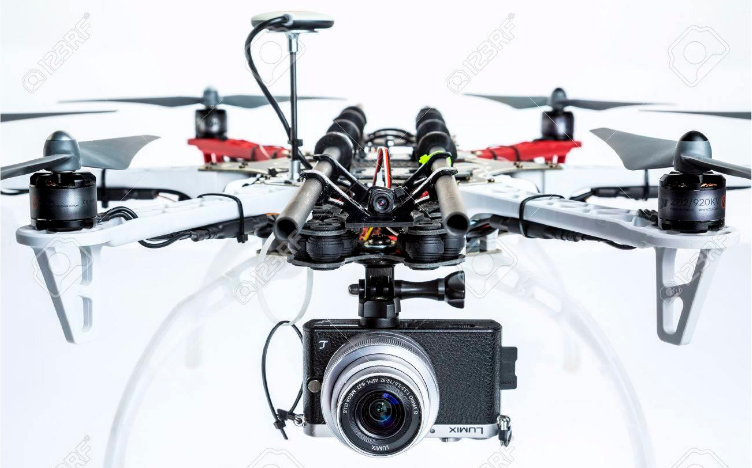
\includegraphics[width=0.8\linewidth]{\figures/FaussePhotoDrone.png}
    \decoRule
    \caption[
    Photo d'un hexacoptère]{
    Photo d'un hexacoptère}
    \label{fig:Photo d'un hexacoptère   }
	\end{figure}


\section{Spécifications techniques}

Malgrès que le projet ai été commencé par un précèdent groupe, la majorité du travail reste à faire (80\%). Leur travail s'appuya sur un cahier des charge, ce dernier nous a été partagé directement, mais sans modification. Le delai, ressources ont changer avec notre équipe. 
Nous avons été amené à réaliser des choix techniques et avons décidé de mettre en faible priorété certaines fonctionnalitées afin de pouvoir rendre une réalisation cohérente dans le temps qui nous a été imposé.

\subsection{Fonctionnalités obligatoires}

L'hexacoptère devra être capable de décoller de manière stabilisé. Cette action devra pouvoir être lancer à partir d'un télécommande. \newline 
Cette dernière devra pouvoir envoyer les ordres de déplacement au drone.  Un retour video sur un écran est envisagé.

\vspace{1cm}
Le drone embarquera une nacelle permettant de supporter et orienté une caméra. \newline
Il disposera d'une caméra permettant de prendre des clichés, et vidéo.

\vspace{1cm}
Concernant le contrôle du drône, une télécommande sera développé afin d'envoyer les ordres de déplacement au drone. La télécommande pourrait un retour vidéo, pour visualisé ce que filme le drone, ou se que le drone prend en photo.

\vspace{1cm}
L'autonomie du drône fait partie des points critique. En fonction des moteurs imposés et de la technologie de baterrie également imposé nous essaierons de rendre le système le plus autonome possible.

\subsection{Fonctionnalités envisagées}

Le vol stabilité et le contrôle manuel de la caméra est envisagé mais ne fairons pas partie des fonctionnalité prioritaire. Elles seront étudier et développé une fois les fonction de base terminé et validé. Tout comme le contrôle de la caméra et le retour vidéo.

\subsection{Matériel}

La base du drone ayant déjà était conçu, nous la réutiliseront. \newline
La carte chargé de la supervision du drone sera une STM32F4. \newline
Le contrôle des moteurs disposera  d'une carte STM32.
Afin de contrôler le dronee à distance la télécommande sera réalisé à partir d'une Raspberry Pi 3, et comme la carte de supervision du drone la Raspberry disposera d'un module émetteur/recepteur radio fréquence. 


\subsection{Résumé des exigences}
\begin{figure}[H]
	\centering
    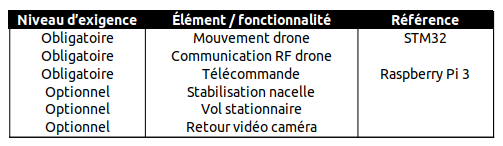
\includegraphics[width=0.7\linewidth]{\figures/tab_exigences.png}
    \decoRule
    \caption[
    Tableau récapitulatif des exigences du projet]{
    Tableau récapitulatif des exigences du projet}
    \label{fig:Tableau récapitulatif des exigences du projet}
	\end{figure}


\section{Organisation}

%outils
%répartition du travail

En tant que groupe de quatre personne, nous avons choisi de travailler en appliquant les méthodes agiles. Ainsi la répartition du travail au sein du groupe se fera de façon dynamique en fonction des aptitudes de chacun et de la charge de travail nécessaire pour terminer une tache donnée en un temps imparti.

\vspace{1cm}

Nous avons sélectionné quelques outils pour travailler de façon optimale~:
\begin{itemize}[label=$\bullet$]
	\item Messenger comme moyen de communication.
	%\item {\href{https://trello.com}{Trello}} comme outil de gestion de projet.
	\item {GitHub comme hébergeur de code source~:\\\url{https://github.com/ThomasAbg/Hexacoptere.git}
	\end{itemize}

\vspace{1cm}

%À l'issue d'une étude technique préliminaire, nous avons dressé un schéma fonctionnel provisoire du système.


%\vspace{1cm}

%Nous avons donc pu trier et organiser les différentes tâches à accomplir et en prioriser certaines représentées en orange sur le diagramme ci-%dessous. Les tâches encadrées de gras sont celles jugées les plus critiques pour l'accomplissement du projet.



